\documentclass[tikz,border=12pt]{standalone}
\usepackage{tikz}
\usetikzlibrary{positioning, arrows.meta, shapes.geometric, calc}

\begin{document}
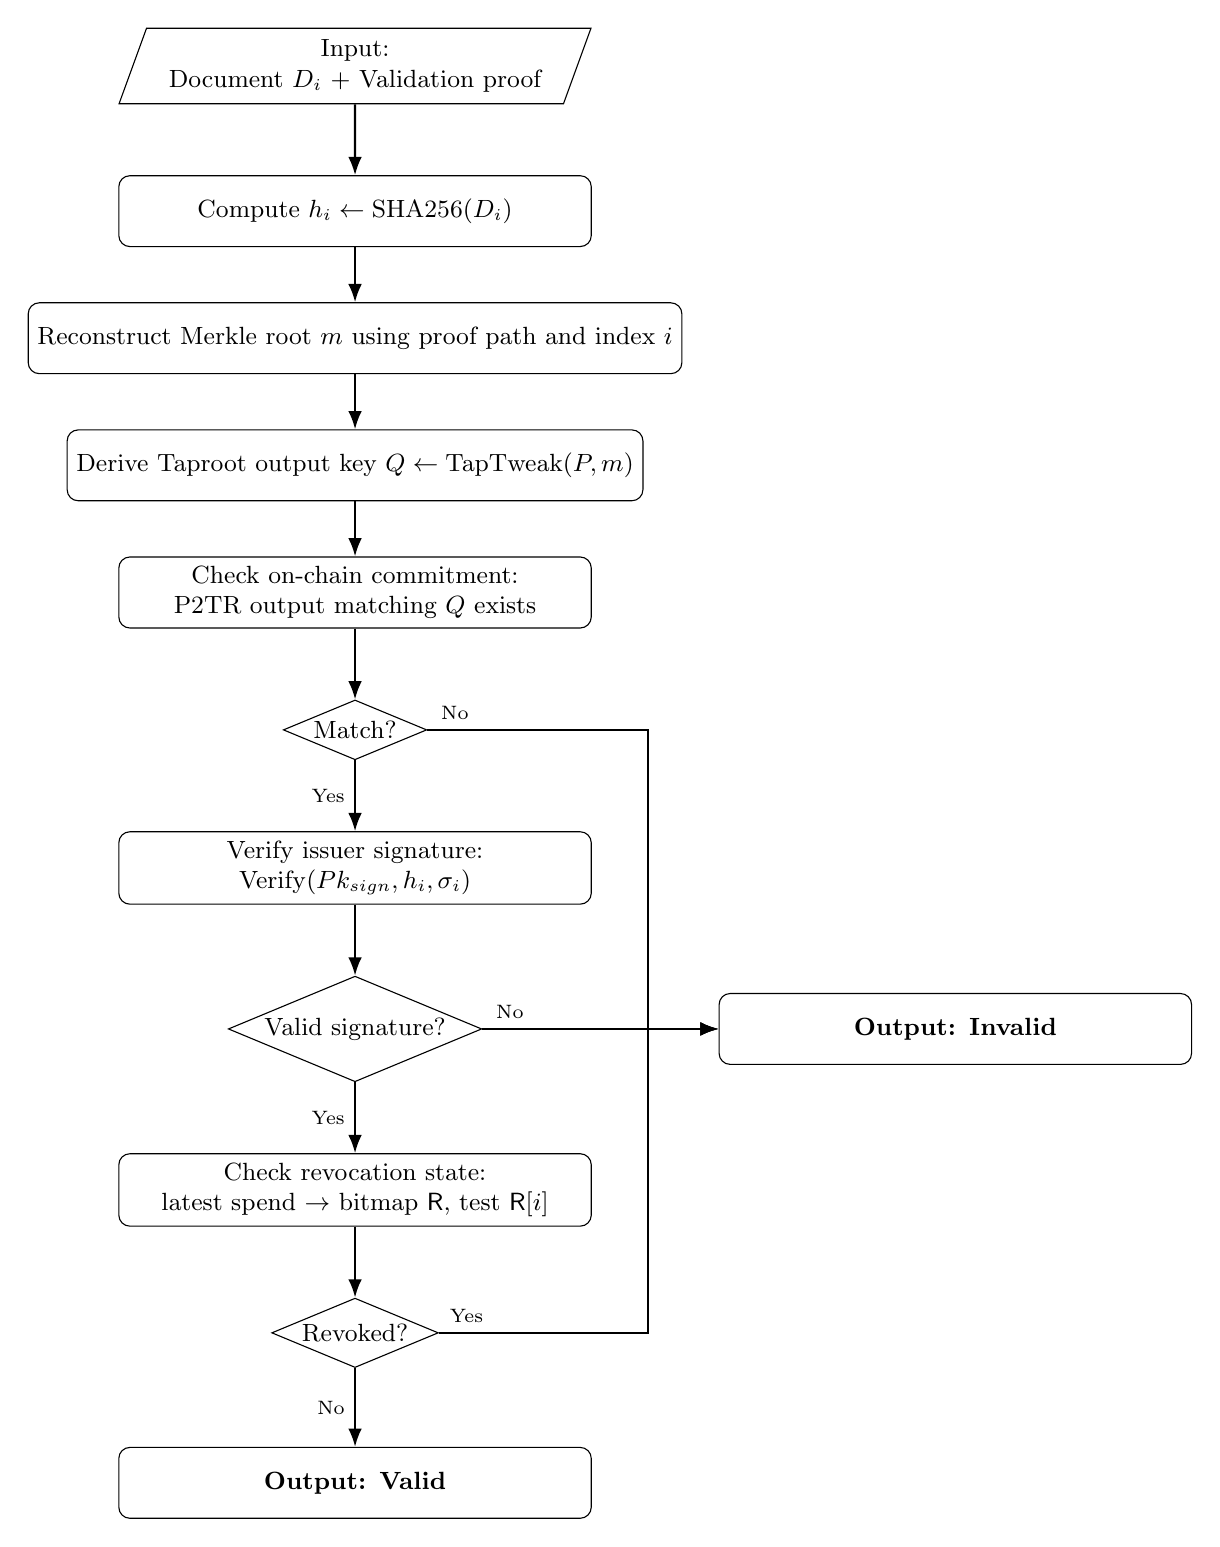
\begin{tikzpicture}[
    font=\small,
    proc/.style={
        draw, rounded corners,
        align=center,
        minimum width=6.0cm,
        minimum height=0.9cm
    },
    io/.style={
        draw, trapezium,
        trapezium left angle=70,
        trapezium right angle=110,
        align=center,
        minimum width=6.0cm,
        minimum height=0.9cm
    },
    decision/.style={
        draw, diamond,
        aspect=2.4,
        align=center,
        inner sep=1pt
    },
    arrow/.style={-Latex, thick},
    note/.style={font=\scriptsize}
]

% ===================== MAIN COLUMN =====================
\node[io] (input) {Input:\\Document $D_i$ + Validation proof};

\node[proc, below=0.9cm of input] (hash)
{Compute $h_i \leftarrow \mathrm{SHA256}(D_i)$};

\node[proc, below=0.7cm of hash] (merkle)
{Reconstruct Merkle root $m$ using proof path and index $i$};

\node[proc, below=0.7cm of merkle] (tap)
{Derive Taproot output key $Q \leftarrow \mathrm{TapTweak}(P,m)$};

\node[proc, below=0.7cm of tap] (chain)
{Check on-chain commitment:\\P2TR output matching $Q$ exists};

\node[decision, below=0.9cm of chain] (d1) {Match?};

\node[proc, below=0.9cm of d1] (sig)
{Verify issuer signature:\\$\mathrm{Verify}(Pk_{sign}, h_i, \sigma_i)$};

\node[decision, below=0.9cm of sig] (d2) {Valid signature?};

\node[proc, below=0.9cm of d2] (rev)
{Check revocation state:\\latest spend $\rightarrow$ bitmap $\mathsf{R}$, test $\mathsf{R}[i]$};

\node[decision, below=0.9cm of rev] (d3) {Revoked?};

\node[proc, below=1.0cm of d3] (valid) {\textbf{Output: Valid}};

% ===================== FIXED "INVALID" COLUMN =====================
% Put Invalid closer and aligned to the middle of the decision stack
\node[proc, right=3cm of d2] (invalid) {\textbf{Output: Invalid}};

% This is a fixed vertical rail (x-position) for all failure branches.
% It is placed to the right of the main column, far enough to never touch blocks.
\coordinate (railTop) at ($(d1.east) + (2.8,0)$);
\coordinate (railBot) at ($(d3.east) + (2.8,0)$);

% ===================== MAIN FLOW ARROWS =====================
\draw[arrow] (input) -- (hash);
\draw[arrow] (hash) -- (merkle);
\draw[arrow] (merkle) -- (tap);
\draw[arrow] (tap) -- (chain);
\draw[arrow] (chain) -- (d1);

\draw[arrow] (d1.south) -- node[left, note]{Yes} (sig);
\draw[arrow] (sig) -- (d2);
\draw[arrow] (d2.south) -- node[left, note]{Yes} (rev);
\draw[arrow] (rev) -- (d3);
\draw[arrow] (d3.south) -- node[left, note]{No} (valid);

% ===================== FAILURE ROUTING (NO CROSSES) =====================
% 1) Draw a thin vertical rail (optional visual guide). Comment out if you want invisible.
% \draw[thick] (railTop) -- (railBot);

% d1: No -> go right to rail, then down to d2-level, then right to invalid
\draw[arrow]
  (d1.east) -- ++(0.35,0) node[above, note]{No}
  -- ($(railTop) + (0,0)$)
  -- ($(railTop |- d2.east)$)
  -- (invalid.west);

% d2: No -> go right to rail at d2-level, then directly to invalid
\draw[arrow]
  (d2.east) -- ++(0.35,0) node[above, note]{No}
  -- ($(railTop |- d2.east)$)
  -- (invalid.west);

% d3: Yes -> go right to rail at d3-level, then up to d2-level, then to invalid
\draw[arrow]
  (d3.east) -- ++(0.35,0) node[above, note]{Yes}
  -- ($(railTop |- d3.east)$)
  -- ($(railTop |- d2.east)$)
  -- (invalid.west);

\end{tikzpicture}
\end{document}
